% This LaTeX was auto-generated from MATLAB code.
% To make changes, update the MATLAB code and export to LaTeX again.

\documentclass{article}

\usepackage[utf8]{inputenc}
\usepackage[T1]{fontenc}
\usepackage{lmodern}
\usepackage{graphicx}
\usepackage{color}
\usepackage{hyperref}
\usepackage{amsmath}
\usepackage{amsfonts}
\usepackage{epstopdf}
\usepackage[table]{xcolor}
\usepackage{matlab}

\sloppy
\epstopdfsetup{outdir=./}
\graphicspath{ {./README_images/} }

\begin{document}

\matlabtitle{Curvas de comportamiento de COVID 19}

\begin{par}
\begin{flushleft}
El comportamiendo de epidemias puede ser simulado con modelos matematicos o modelos estadisticos. En este estudio nos concentraremos en los modelos matematicos. Especificamente usaremos un modelo \textbf{compartimental}. Los modelos de este tipo simplifican el problema al dividir la poblacion total en compartimentos, asumiendo que cada individuo en un mismo compartimento tiene las mismas características.
\end{flushleft}
\end{par}

\matlabheading{Requisitos}

\begin{par}
\begin{flushleft}
Para simular el comportamiento de la epidemia usaremos el modelo \textbf{SIR }(\textbf{S}usceptible \textbf{I}nfectious \textbf{R}emoved). El modelo consiste de tres compartimiendos
\end{flushleft}
\end{par}

\begin{itemize}
\setlength{\itemsep}{-1ex}
   \item{\begin{flushleft} \textbf{S}: Personas susceptibles. Estos se pueden pasar al grupo de \textbf{I}nfectados al tener contacto con uno de ellos. \end{flushleft}}
   \item{\begin{flushleft} \textbf{I}: Personas infectadas. Aquellos que son portadores de la enfermedad. \end{flushleft}}
   \item{\begin{flushleft} \textbf{R}: Personas con inmunidad o que murieron. Este grupo puede ser interpretado de varias formas, pero son aquellas que fueron infectadas y ya no pertenecen a ese grupo. \end{flushleft}}
\end{itemize}

\begin{par}
\begin{flushleft}
Usaremos el modelo y modificaremos las variables necesarias para asimilar diferentes cepas de covid, asi como diferentes tamaños de población y la densidad de estas.
\end{flushleft}
\end{par}

\begin{par}
\begin{flushleft}
Al final compararemos nuestras gráficas de variables continuas contra las variables discretas y veremos que similitudes y diferencias se creán entre la realidad y este modelo matematico simple.
\end{flushleft}
\end{par}

\matlabheading{Creación del modelo}

\begin{par}
\begin{flushleft}
Usaremos el modelo \textbf{SIR} de acuerdo al siguiente sistema de ecuaciones:
\end{flushleft}
\end{par}

\begin{par}
$$\begin{array}{l}
\frac{\mathrm{dS}}{\mathrm{dt}}=-\beta \cdot \mathrm{S}\cdot \mathrm{I}+\delta \cdot \mathrm{R}\\
\frac{\mathrm{dI}}{\mathrm{dt}}=\beta \cdot \mathrm{S}\cdot \mathrm{I}-\gamma \cdot \mathrm{I}\\
\frac{\mathrm{dR}}{\mathrm{dt}}=\gamma \cdot \mathrm{I}-\delta \cdot \mathrm{R}
\end{array}$$
\end{par}

\begin{par}
\begin{flushleft}
Aqui $\beta \cdot \mathrm{S}\cdot \mathrm{I}$ representa la cantidad de personas que es contagiada, es decir, los que pasan de ser susceptibles a ser contagiados (infectados). Es por esto que la constante $\beta$ (beta) representa la taza de infección. Se sabe que unas cepas de covid son más infeccionsas que otras.
\end{flushleft}
\end{par}

\begin{par}
\begin{flushleft}
De la misma forma $\delta$ representa la perdida de inmunidad. Por eso $\delta \cdot \mathrm{R}$ representa a aquellos que pasan del compartimiento de removed, a ser susceptibles otra vez, es decir que pueden volverse a infectar.
\end{flushleft}
\end{par}

\begin{par}
\begin{flushleft}
Por último $\gamma$(gamma) representa la taza de recuperación.
\end{flushleft}
\end{par}

\begin{par}
\begin{flushleft}
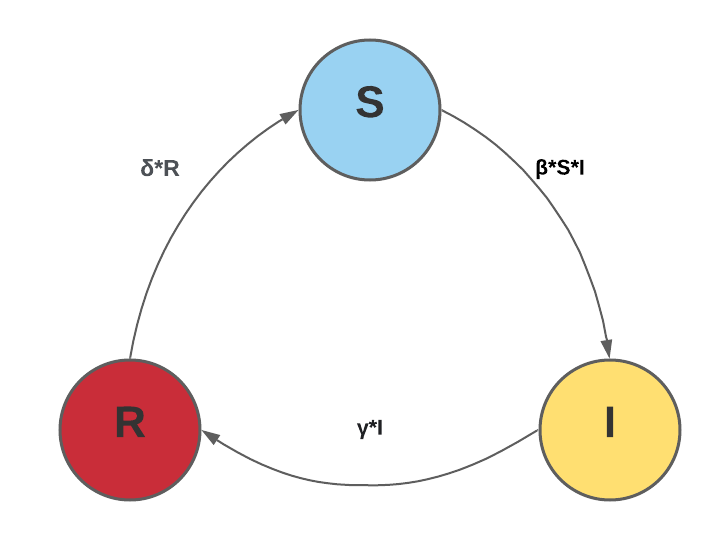
\includegraphics[width=\maxwidth{45.05770195684897em}]{image_0}
\end{flushleft}
\end{par}

\begin{par}
\begin{flushleft}
    \textbf{Figura 1: }Diagrama de flujo del model SIR
\end{flushleft}
\end{par}


\vspace{1em}
\matlabheading{Implementación}

\begin{matlabcode}
% Model parameters
beta = 5*10^-9; % rate of infection
gamma = 0.12; % rate of recovery (try also 0.07)
delta = 0.0; % rate of immunity loss
N = 6*10^7; % Total population N = S + I + R
I0 = 10; % initial number of infected
T = 300; % period of 300 days
dt = 1/4; % time interval of 6 hours (1/4 of a day)
fprintf('Value of parameter R0 is %.2f',N*beta/gamma)
\end{matlabcode}
\begin{matlaboutput}
Value of parameter R0 is 2.50
\end{matlaboutput}
\begin{matlabcode}
[t,S,I,R] = modelSIR(beta,gamma,delta,N,I0,T,dt);
% Plots that display the epidemic outbreak
% Curve
plot(t,S); 
hold on
plot(t,I); 
plot(t,R); 
grid on;
xlabel('Days'); 
ylabel('Number of individuals');
legend('S','I','R');
hold off
\end{matlabcode}
\begin{center}
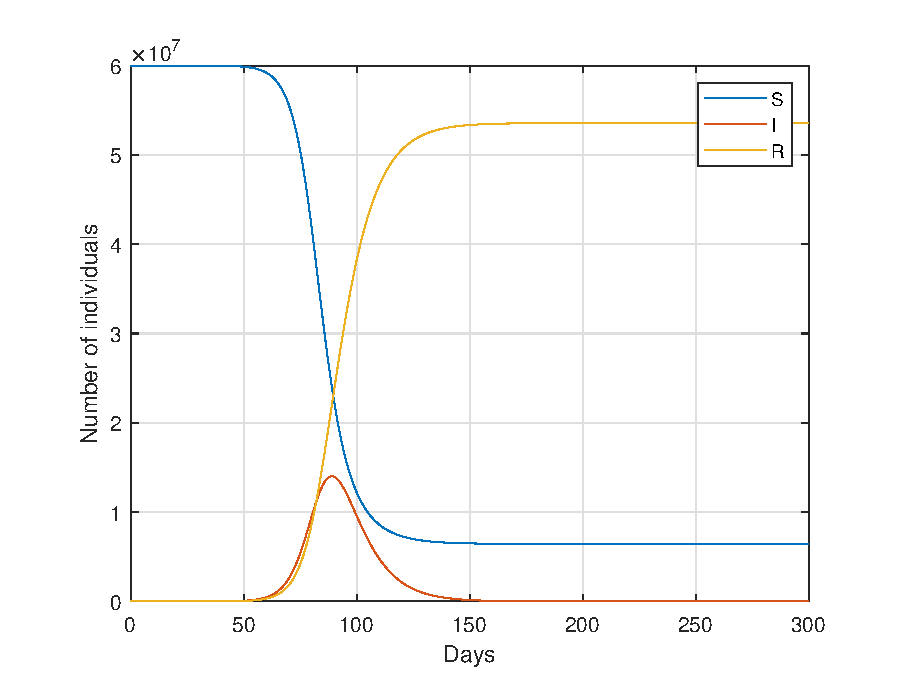
\includegraphics[width=\maxwidth{56.196688409433015em}]{figure_0.eps}
\end{center}

\matlabheading{Pruebas y resultados}

\matlabheading{Conclusión}

\begin{matlabcode}
% x
\end{matlabcode}


\matlabheading{Funciones}

\begin{matlabcode}
function [t,S,I,R] = modelSIR(beta,gamma,delta,N,I0,T,dt)
    [t,y] = runKut4(@(t,y) SIRfunc(t,y,beta,gamma,delta),0,dt,T,[N-I0;I0;0]);    
    S=y(:,1);
    I=y(:,2);
    R=y(:,3);
end

function [xSol,ySol] = runKut4(F,x0,h,xStop,y0)
    % 4th-order Runge--Kutta integration.
    % USAGE: [xSol,ySol] = runKut4(dEqs,x,y,xStop,h)
    % INPUT:
    % dEqs = handle of function that specifies the    
    % 1st-order differential equations
    % F(x,y) = [dy1/dx dy2/dx dy3/dx ...].
    % x,y = initial values; y must be row vector.
    % xStop = terminal value of x.
    % h = increment of x used in integration.
    % OUTPUT:
    % xSol = x-values at which solution is computed.
    % ySol = values of y corresponding to the x-values.
    reshape( y0, [],1 ); % column vector
    xSol = zeros(2,1); 
    ySol = zeros(length(y0),2);
    xSol(1) = x0; 
    ySol(:,1) = y0;
    i = 1;
    x=x0;
    y=y0;    
    while x < xStop
        i = i + 1;
        h = min(h,xStop - x);
        K1 = h*F(x,y);
        K2 = h*F(x + h/2,y + K1/2);
        K3 = h*F(x + h/2,y + K2/2);
        K4 = h*F(x+h,y + K3);
        y = y + (K1 + 2*K2 + 2*K3 + K4)/6;
        x = x + h;
        xSol(i) = x;
        ySol(:,i) = y; 
    end
    
    xSol = xSol';
    ySol=ySol';
end

function dydt = SIRfunc(t,y,beta,gamma,delta)
    dydt = zeros(3,1);
    %dydt(1)=dS
    %dydt(2)=dI
    %dydt(3)=dR
    dydt(1) = (-beta.*y(2).*y(1) + delta.*y(3));    
    dydt(2) = (beta.*y(2).*y(1) - gamma.*y(2));
    dydt(3) = (gamma.*y(2) - delta.*y(3));
end


\end{matlabcode}

\end{document}
